\documentclass[1p]{elsarticle}

\usepackage{amsmath}
\usepackage{amssymb}
\usepackage{graphicx}
\usepackage[colorlinks,unicode,linkcolor=black]{hyperref}
\usepackage{listings}
\lstset{
    language=C++,
    basicstyle=\small,
    %numbers=left,
    columns=flexible,
    %extendedchars=false,
    showstringspaces=false,
    %texcl=true,
    frame=shadowbox
    }
\newcommand{\code}[1]{\lstinline|#1|}
\newcommand{\figref}[1]{Fig.~\ref{#1}}

\journal{Journal of Parallel and Distributed Computing}

\begin{document}

\begin{frontmatter}

\title{Programming OpenCL and CUDA:\\a Case Study Using Modern C++ Libraries}

\author{Karsten Ahnert}
\ead{kahnert@uni-potsdam.de}
\address{
Institut f\"ur Physik und Astronomie, Universit\"at Potsdam,\\
Karl-Liebknecht-Strasse 24/25, 14476 Potsdam-Golm, Germany
}

\author{Denis Demidov}
\ead{ddemidov@ksu.ru}
\address{
Kazan Branch of Joint Supercomputer Center,
Russian Academy of Sciences,\\
Lobachevsky st. 2/31, 420008 Kazan, Russia
}

\begin{abstract}
    We present comparison of several modern C++ libraries intended for OpenCL
    and CUDA programming. The comparison is based on odeint~--- framework for
    solution of ordinary differential equations. Odeint is designed in a very
    flexible way such that the algorithms are completely independent from the
    underlying containers and even from the basic algebraic computations. This
    allows to effectively use such libraries as VexCL, ViennaCL or Thrust to
    solve ODEs with either OpenCL or CUDA technologies. We found that OpenCL
    and CUDA work equally well for problems of large sizes, although OpenCL is
    not well suited for smaller problems due to its higher initialization
    overhead.
\end{abstract}

\begin{keyword}
    GPGPU \sep OpenCL \sep CUDA \sep Modern C++ libraries
\end{keyword}

\end{frontmatter}

\section{Introduction}

Recently, GPGPU based computing has acquired considerable momentum in
scientific community. This is confirmed both by increasing numbers of
GPGPU-related publications and GPU based supercomputers in
top500\footnote{\href{http://top500.org/}{http://top500.org/}} list. Major
programming frameworks are NVIDIA CUDA and OpenCL.  The former is proprietary
parallel computing architecture developed by Nvidia for general purpose
computing on Nvidia graphics cards, and the latter is open, royalty-free
standard for cross-platform, parallel programming of modern processors backed
by Khronos group. The frameworks have their distinctive pros and cons. CUDA has
more mature programming environment with larger set of scientific libraries;
but it is only supported on NVIDIA hardware. OpenCL is an open standard
supported on wide range of hardware but it requires much larger amount of
boilerplate code from a developer.

This paper presents comparison of OpenCL and CUDA performance in the context of
solving ordinary differential equations. The comparison is based on odeint~---
modern C++ library for solution of ODEs. Odeint is designed in a very flexible
way such that the algorithms are completely independent from the underlying
containers and even from the basic algebraic computations. This allows to
effectively use libraries implementing basic linear algebra operations with
either OpenCL or CUDA technologies for solution of ODEs.

\section{Libraries used in comparison}

\subsection{Odeint}

Odeint\footnote{\href{http://odeint.com}{http://odeint.com}}
is a modern C++ library for numerically solving Ordinary Differential
Equations. It is developed in a generic way using Template Metaprogramming
which leads to extraordinary high flexibility at top performance. The numerical
algorithms are implemented independently of the underlying arithmetics. This
results in an incredible applicability of the library, especially in
non-standard environments. For example, odeint supports matrix types, arbitrary
precision arithmetics and can be easily adopted to use either CUDA or OpenCL
frameworks.

In this work odeint is used as a basis for comparison of CUDA and OpenCL
libraries.

\subsection{Thrust}

Thrust%
\footnote{\href{http://thrust.github.com}{http://thrust.github.com}}
is a parallel algorithms library which resembles the C++ Standard Template
Library. Thrust's high-level interface greatly enhances developer
productivity while enabling performance portability between GPUs and multicore
CPUs. Thrust is distributed with NVIDIA CUDA Toolkit since version 4.1.

\subsection{VexCL}

VexCL%
\footnote{\href{https://github.com/ddemidov/vexcl}{https://github.com/ddemidov/vexcl}}
is vector expression template library for OpenCL. It has been created for ease
of OpenCL developement with C++.  VexCL strives to reduce amount of boilerplate
code needed to develop OpenCL applications. The library provides convenient and
intuitive notation for vector arithmetic, reduction, and sparse matrix-vector
multiplication. Multi-device and even multi-platform computations are
supported. 

\subsection{ViennaCL}

The Vienna Computing Library%
\footnote{\href{http://viennacl.sourceforge.net}{http://viennacl.sourceforge.net}}
(ViennaCL) is a scientific computing library written in C++ and based on
OpenCL. It allows simple, high-level access to the vast computing resources
available on parallel architectures such as GPUs and is primarily focused on
common linear algebra operations (BLAS levels 1, 2 and 3) and the solution of
large systems of equations by means of iterative methods with optional
preconditioner.

%Odeint supports Thrust and VexCL natively, but for ViennaCL we needed to
%provide adaptation code. Since ViennaCL already supports expression templates
%it can directly be used with the \code{vector_space_algebra} of odeint. There
%is no need to introduce an additional algebra or new operations. So in order to
%use \code{viennacl::vector} with odeint we only only needed to adapt the
%resizing operation. Resizing in odeint is necessary since many solvers need
%temporary state types. These state types need to be constructed and initialized
%which is done by the resizing mechanism of odeint.
%
%The resizing mechanism of odeint consist of three class templates. These
%classes are \code{is_resizeable<>} which is simply a meta function telling
%odeint if the type is really resizable. The second class is
%\code{same_size_impl<>} which has a static method \code{same_size} taking two
%\code{state_type} instances as arguments and returning if both instances have
%the same size. The third class is \code{resize_impl<>} which performs the
%actual resizing. These classes have a default implementation and can be
%specialized for any type.  For ViennaCL the specialization is very simple and
%is presented on \figref{fig:adapt:viennacl}.
%
%We were only able to test damped harmonic oscillator example with ViennaCL,
%since the library lacks such vector operations as elementwise multiplication or
%function application necessary for the other examples.  Nevertheless we
%consider comparison with ViennaCL interesting enough to include in this paper.
%Indeed, ViennaCL and VexCL employ somewhat different approaches to OpenCL
%kernel generation. ViennaCL has limited number of kernels, which coincide
%functionally with BLAS level 1 routines. These kernels are compiled in batch at
%the program start to allow for faster initialization. However, due to this
%design decision each vector expression may result in launch of more than one
%kernel.  On the other hand, VexCL generates and compiles single kernel for each
%vector expression it encounters.  This leads to higher initialization overhead,
%but should prove more effective in the long runs. It should be noted that main
%aim of ViennaCL is provision of iterative solvers for large sparse systems of
%equations. In this context complex vector expressions are rare and we think
%that authors of ViennaCL made correct design decision.  However, we think it is
%interesting to compare approaches of VexCL and ViennaCL.

\section{Numerical experiments}

\subsection{Lorenz Attractor Ensemble}

In the first example we will use the Lorenz system and study its dependence on
one of the parameters. The Lorenz system is a system of three coupled ODEs
which shows chaotic behavior for a large range of parameters. The ODE reads
\begin{align}
    \frac{dx}{dt} &= -\sigma \left( x - y \right), \\
    \frac{dy}{dt} &= R x - y - xz, \\
    \frac{dz}{dt} &= -bz + xy.
\end{align}

We will study the dependence on the parameter $R$. Therefore, we create a large
set of these systems (each with a different parameter $R$), pack them all into
one system and solve them simultaneously on the GPU.

\subsection{Chain of Coupled Phase Oscillators}

As a second example we choose a chain of coupled phase oscillators. Phase
oscillators are a very simplified version of usual oscillator where the state
is described by a $2\pi$ periodic variable. If a single phase oscillator is
uncoupled its phase $\phi$ is described by a linear growth $d\phi/dt = \omega$
where $\omega$ is the phase velocity. Therefore, interesting behavior can only
be observed if two or more oscillators are coupled. In fact, a system of
coupled phase oscillators is a prominent example of an emergent system where
the coupled system shows a more complex behavior than its constitutes.

The concrete example we analyze here is:
\begin{equation}
    \frac{d\phi_i}{dt} = \omega_i + \sin( \phi_{i+1} - \phi_i) + \sin( \phi_i
    - \phi_{i-1}).
\end{equation}
Note that $\phi_i$ is a function of the time, the index $i$ denotes here the
$i$-th phase in the chain.

\subsection{Damped Harmonic Oscillator Ensemble}

Some words about odeint\footnote{\href{http://odeint.com}{http://odeint.com}}
and steps required to solve an ODE with libraries below.

\section{Results}

\subsection{Lorenz Attractor Ensemble}

\begin{figure}
    \begin{center}
	\includegraphics[width=\textwidth]{data/lorenz_ensemble/perfcmp}
    \end{center}
    \caption{Lorenz attractor ensemble results}
    \label{fig:lorenz:perf}
\end{figure}

\subsection{Chain of Coupled Phase Oscillators}

\begin{figure}
    \begin{center}
	\includegraphics[width=\textwidth]{data/phase_oscillator_chain/perfcmp}
    \end{center}
    \caption{Phase oscillator chain results}
    \label{fig:phase:perf}
\end{figure}

\subsection{Damped oscillator ensemble}

\begin{figure}
    \begin{center}
	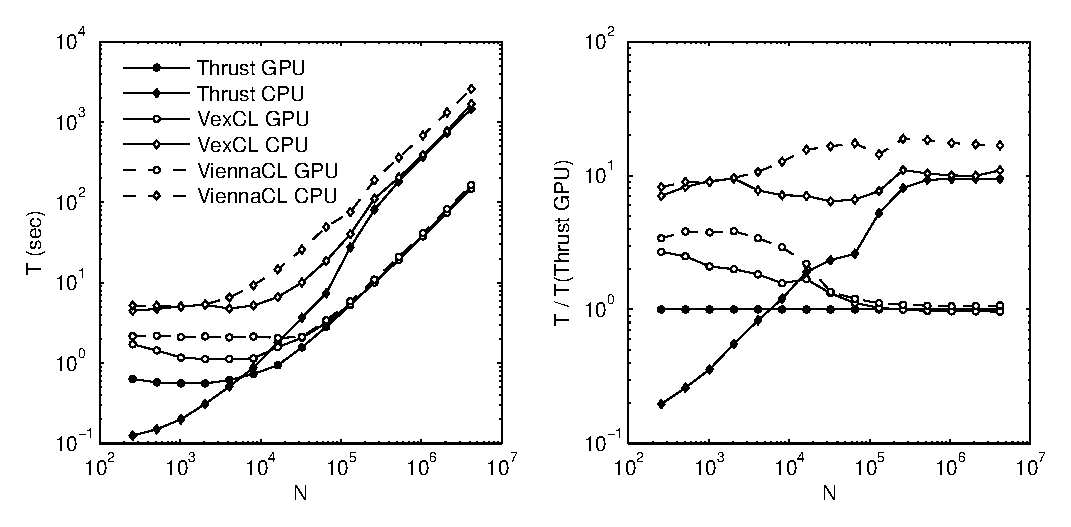
\includegraphics[width=\textwidth]{data/damped_oscillator/perfcmp}
    \end{center}
    \caption{Damped oscillator ensemble results}
    \label{fig:phase:perf}
\end{figure}

\subsection{Disordered Ham Lattice}

\begin{figure}
    \begin{center}
	\includegraphics[width=\textwidth]{data/disordered_lattice/perfcmp}
    \end{center}
    \caption{Disordered Ham lattice results}
    \label{fig:phase:perf}
\end{figure}

\section{Conclusion}

\section{Acknowledgments}

This work has been partially supported by RFBR grant No 12-07-0007.

\nocite{*}
\bibliographystyle{model1-num-names}
\bibliography{ref}

\end{document}
